\chapter{Local Training}

\section{Local Training vs. Cloud Training}
Author: Sebastian Rohrer\newline
One of the major drawbacks of using the DeepRacer in a learning environment is the costs of training. Amazon offers easy, albeit functionally limited, ways of training RL models in their cloud services. This contradicts the intended use, as the DeepRacer is supposed to offer a simple and affordable entry into the ways of machine learning.
 To circumvent this cost barrier, we -- like others before us -- began setting up a training environment on one of the more powerful computers in the robotics lab. After searching the internet we found a very cost-efficient method, to train the model on our computer. Given that we gain access to a "super-computer" in our robotics lab, which would train our models easily and fast, we decided to train it by ourselves. Amazon does not provide an easy to use interface to download and upload models because they do not want to support the end user using his own servers and computers to train. Following this idea, many people worked their way around and made their own GUI's and interfaces.
 The setup for local training is available on GitHub. 

\subsection{Prerequisites}
\footcite{https://github.com/aws-deepracer-community/deepracer}. In order to function properly the computer had to meet the following requirements:

\begin{itemize}
 \item Docker + Docker Compose
 \item vncviewer 
 \item Nvidia CUDA/cuDDN 
 \item Minio
 \item Python
\end{itemize}

\subsection{Docker}

\subsubsection{Docker}
Docker is free to use software that isolates applications using container virtualisation. It simplifies application deployment because the container containing all the necessary packages, and package dependencies, can be easily transferred and mapped into a so-called Docker image. The container ensures that the resources used on the computer are separated and managed. This includes: code, runtime-modules, system tools, system-libraries etc.\repeatfootcite{Docker-Compose}

\subsubsection{Docker-Compose}
Compose is a tool used to handle multiple Docker images. Using a Yet Another Multicolumn Layout(YAML)-File, all the services and application needs can be configured. Then with only one command, all the files and services from the configuration can be started.

\subsubsection{YAML}
Yet Another Multicolumn Layout(YAML), a super-set of JSON, is a human-readable language used for the serialisation of data. Its most common use is in data files, in which data is stored and transmitted to an application. It targets the same communication applications as the Extensible Markup Language(XML). \repeatfootcite{YAML}

\subsection{VNC-Viewer}

\subsubsection{VNC}
In computing, virtual network computing (VNC) is a platform-independent, graphical desktop sharing system that uses the remote frame buffer protocol (RFB) to control another computational system remotely. It gets differentiated between a VNC-Client and VNC-Server; multiple Clients can connect to the same server.

\subsubsection{RFB}
The Remote Frame-buffer Protocol(RFB) is a TCP Network protocol using the Port 5900 + Desktop Number. Its main task is to transfer data such as screen-contents and user-inputs.\repeatfootcite{RFB}

\subsubsection{VNC-Viewer}
VNC-Viewer is the Program, which allows the Client to connect to a server and remotely control it. On the other side, the server will run a VNC-Server application.\repeatfootcite{VNC/VNC-Viewer}


\subsection{Nvidia CUDA/CUDDN}

\subsubsection{CUDA}
CUDA (previously known as Compute Unified Device Architecture) is a programming technology developed by Nvidia that allows part of the Program to be processed by a graphics processing unit (GPU). Providing additional computing power in GPU is necessary for a highly parallelisable program sequence (high data parallelism) because the GPU is usually much faster than the CPU. CUDA is mainly used for scientific and technical computing. CUDA is usually programmed in C, although multiple wrappers for other languages like Ruby, Python or Java exist.\repeatfootcite{Nvidia-CUDA}

\subsubsection{cuDDN}
Nvidia cuDDN(CUDA Deep Neural Network) is a library used for GPU accelerated deep neural network learning. It provides highly optimised implementations for routines, like pooling, forward and backward convolution, normalisation and activation layers.\repeatfootcite{Nvidia-cuDDN}

\subsection{Minio}
Minio is a popular High-Performance open source-based object storage server. It's optimised to be used with the Amazon S3 cloud storage service. It can be used it to build a performance-based infrastructure for machine learning, application data workloads and analytics. If more control over the object storage server is needed, applications ca be configured to communicate with Amazon S3 to make Minio an alternative to Amazon.

\subsection{Python}

\subsubsection{Why use Python?}
All the Amazon services provide an API that is used to communicate between them. Python3 is used in all scripts to build and establish a connection and handle the user-defined functions. The Artificial Intelligence itself is also coded in Python. Therefore it's the easiest and quickest way to write Code and extend the existing Codebase in Python. The rising number of Machine Learning Library's for Python is one of the key points why Amazon decided to code in this language.

\subsubsection{Python}
Python is a low-level Programming-Language used in many different use-cases. It's easy to learn and has very good documentation. It is required to have a Python installation, because the local training solutions are all coded in Python. \repeatfootcite{Python}

\section{Amazon tools}
To train and create the model according to the rules, it is necessary to use Services provided by Amazon. The major tools we used in our project were:

\begin{itemize}
    \item Sagemaker
    \item Robomaker
    \item S3
\end{itemize}


\section{Other Tools}
These Tools are getting installed automatically when the init.sh Script is run as explained below. The most important two are Gazebo and rviz.

\subsection{Gazebo}
Gazebo is a 3-Dimensional open-source Robotics and Physics Simulator. It integrates the ODE Physics engine, OpenGL rendering and also supports sensor and actuator control. Gazebo uses multiple high-performance realistic physics engines like Bullet. It provides environment rendering like lighting, shadows and textures.\repeatfootcite{Gazebo} 

\subsection{rviz}
ROS Visualisation (rviz) is a graphical user interface based on the Robot Operating System(ROS), that outputs images and videos. This use-case acts as the Visual Component on which it is possible to see the training progress and the Deepracer. Gazebo simulates the Progress and the Physics and then sends the processed output to rviz, which replicates the video stream. Based on the shown output, the hyperparameter can be adjusted to get better performance.\repeatfootcite{rviz}

\section{Implementing the local training methods}

\subsection{Deepracer-Wiki}
Although most of the Information about the Deepracer and The Amazon Deepracer League is in the Online Management Console of Amazon, some users made an own independent Deepracer-Wiki. Much Information can be found for local training, parameter adjustment and vehicle hacking. It also links to a community blog, a community website and a general community-GitHub page. \repeatfootcite{Deepracer-Wiki}

\subsubsection{Local-Training Solutions}
The Wiki includes an entire list of 6 different documented GitHub projects from users who tried to locally install all the amazon services and set up a whole local training environment. We tried two different Repository is in our installation process because the first one did not work as expected on the PC. More Information about the process will be in the next section.

\subsection{First Approach}
The first approach was to clone a GitHub repository, which implemented the whole algorithm and a graphical user interface. The author of this project relies heavily on another repository from the GitHub user crr0004\repeatfootcite{Local-Training-1}. Because his instructions were unclear and the project itself lacked features and had poor usability, he decided to expand the project and make it easier to use. 
Before getting started with the installation, the local machine has to meet the prerequisites:
First, ensure that the operating system is Ubuntu 18.04 or higher because some of the packages needed are only available on Linux.
The next main point is to check if the system runs on an Nvidia GPU and has CUDA/CUDNN installed and configured. If the machine does not integrate an Nvidia GPU, it is only possible to train on the CPU, which is much slower and takes more time.
Docker is also needed as well as the Nvidia-Docker runtime. This is used for the training environment to gain access to the GPU and create new timelines.
Lastly, vncviewer has to be installed because it is the program that controls all interaction between the graphical user interface and the controllers from amazon.
If the system meets all the requirements above the init.sh script from the GitHub repository has to be executed.
This may take up to 10 minutes, and all it does is, it clones crr0004's repository, runs the required scripts and creates the necessary folder structure, including all the needed files, to manually adjust the code, train the model, and upload it to amazon.
After the installation and initialisation process is completed, we could start a training session, but after about 10 minutes, the program crash. Searching the internet, we did not find any evidence that we made errors during the installation process, and we also were not able to fix them.

\subsection{Final Approach}
The second try was to download Matt Camps\repeatfootcite{Local-Training-2} solution, which relies heavily on crr0004's GitHub repository, but it has more detailed instructions and does not use as many self-programmed scripts. The only Prerequisites the computer has to have installed are the Nvidia CUDA drivers and docker-compose. That made it easy to install and debug if errors occurred. The next step was to clone the Repository and run the init.sh. However, following the tutorial, we were not able to start a training session. After debugging and logging, we found out that the project heavily relies on Amazon Sagemaker, but the corresponding docker image was never pulled and installed. After downloading it, the scripts ran flawlessly, and no following errors occurred.

\section{Training and setup process}

\subsection{Installation Guide}
After our successful installation, this is a complete manual of the installation process. \newline Before the beginning, the system has to have all the prerequisites installed.\repeatfootcite{Local-Training-2}

\begin{enumerate}
    \item At first, the docker-nvidia2 has to be set as the default runtime in the daemon.json file that's located in /etc/docker/.
    \newline The argument \textsl{default-runtime} should beset to \textsl{nvidia} 
    \item The next step is to install Amazon Sagemaker. Use the Command \textsl{sudo apt-get install Sagemaker}  to download it from the Ubuntu packet-manager. This is necessary, because the following code will depend on the provided API from the Package.
    \item Completing the installation clone the GitHub Repository\url{https://github.com/mattcamp/deepracer-local/} and run the \textsl{start-training.sh} Script.
\end{enumerate}


\subsection{Folder structure}
In the Main-Folder, called deepracer-local are all files needed, to train the model.
The most important scripts are:

\begin{itemize}
    \item start-training.sh
    \item stop-training.sh
    \item delete-last-run.sh
    \item upload-current.sh
    \item mk-model.sh
    \item local-copy.sh
\end{itemize}

\subsubsection{start-training.sh}
The start-training.sh Shell Script starts a new Training-Session. The model data directory must be empty because the current progress is saved there. If a already trained model should be improved, the following parameter has to be set in the file hyperparams.json; "pretrained": "true". When starting for the first time, it will download 10GB of docker images; therefore, it will take a while to start the training process.

\subsubsection{stop-training.sh}
This Script stops the current Training. If running, it will take at least 20s to stop because it will first stop Sagemaker, then it sleeps till Robomaker creates a model.tar.gz in which the model data from the current model is stored, and then it will stop completely. In this Format, it is ready to be uploaded on a physical Deepracer.

\subsubsection{delete-last-run.sh}
Clears the current bucket to prepare the model data directory to start a new training session.

\subsubsection{upload-current.sh}
Loads current model files into a Model directory that the user can specify before.

\subsubsection{mk-model.sh}
Creates a complete model from the training model that can be uploaded to a physical car.

\subsubsection{local-copy.sh}
Copies the currently trained model data to a save directory. This command must be executed before the delete-last-run.sh script; otherwise, all model data will be lost.

other important files that change regularly are:

\begin{itemize}
    \item hyperparams.json
    \item config.env
    \item custom-files directory
    \item reward.py
\end{itemize}

\subsubsection{hyperparams.json}
Includes the Hyperparameters that can be changed, such as batch size, loss rate and a number of epochs.

\subsubsection{config.env}
Stores the Training Parameters and the track name. The track name has to be the same as in the training-params.yaml file.

\subsubsection{reward.py}
Stores the reward function that the user can change. This is the most important file and is changed the most.

\subsection{starting a training session}
Starting a new training session, a decision must be made, whether to create a new model within the session or use a pretrained model and improve the performance.
\newline If a new model is to be created, first-run delete-last-run, then start-training. This will output the current training parameters and a number of epochs.
\newline More often, a pretrained model is used to train run the local-copy before and change the "pretrained" parameter in the hyperprams.json to true and then follow the instructions as explained above.

\begin{figure}[H]
    \centering
    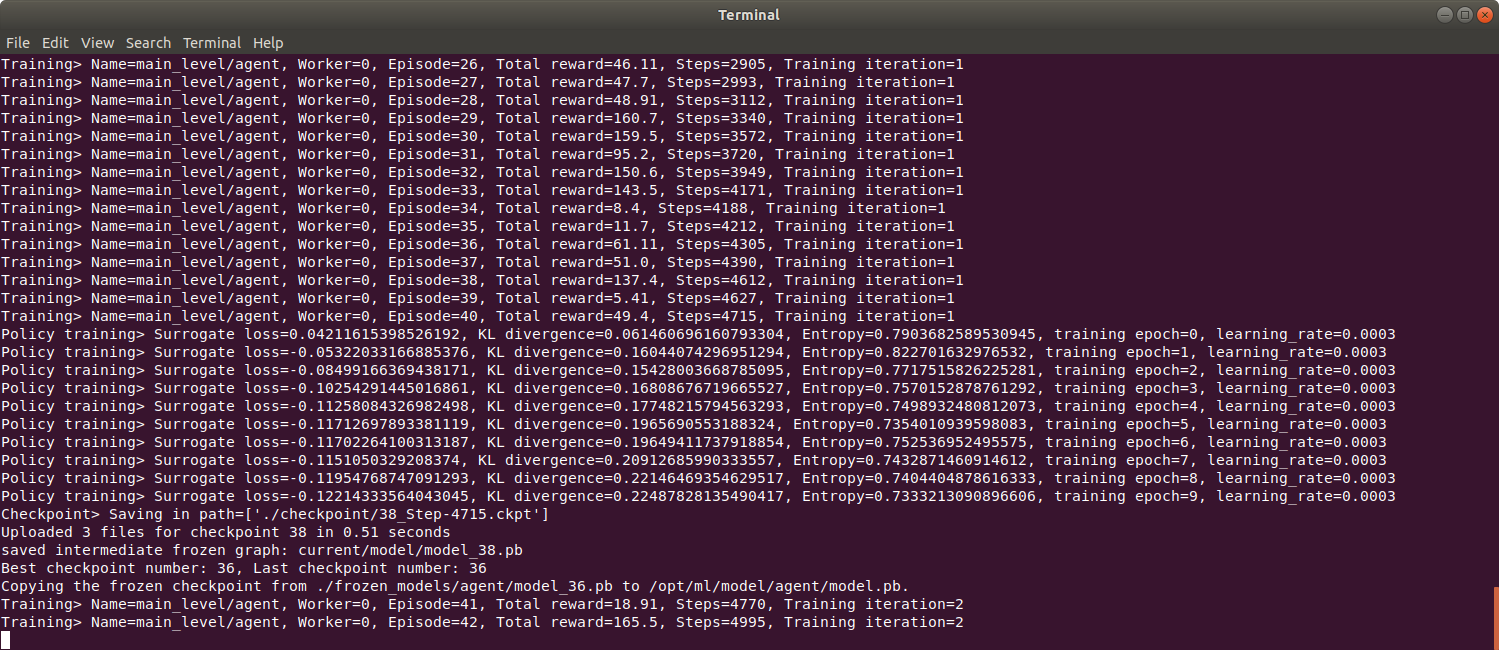
\includegraphics[width=0.9\textwidth]{images/deepracer_local_session1_1_console.png}
    \caption[]{Output from start-training\footnotemark}
    \label{fig:console-output-start}
\end{figure}

If the session is completed, use stop-training. This will take between 20 and 25 seconds. When the stopping process is completed, the model should be copied into a save directory via the script local-copy.sh. Completing the whole progress, run mk-model and get the finished model, to upload it to the Deepracer.

\begin{figure}[H]
    \centering
    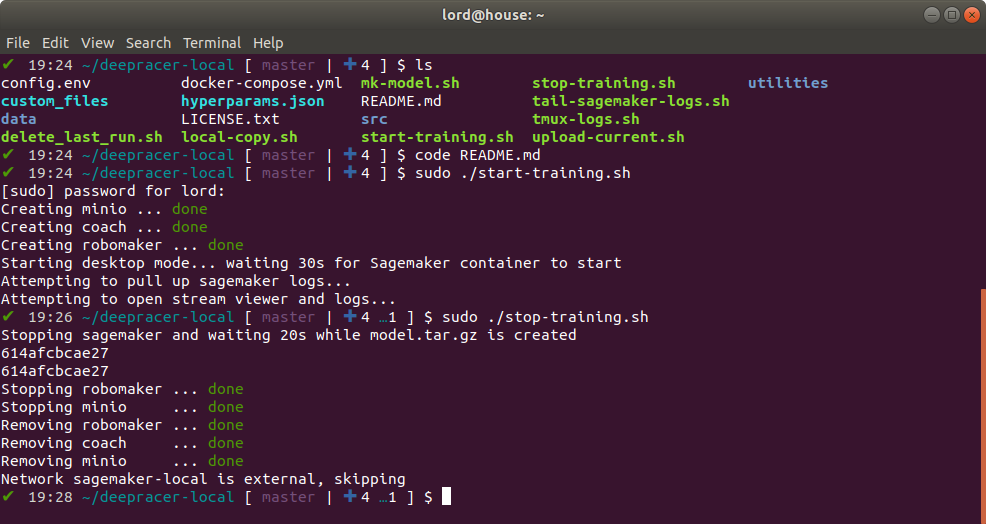
\includegraphics[width=0.9\textwidth]{images/deepracer_local_training_stop.png}
    \caption[]{Output from stop-training\footnotemark}
    \label{fig:console-output-stop}
\end{figure}

\section{Errors occurring during the Installation process}
On our first try, we installed all the required tools and services but made a mistake to forget to specify the Nvidia CUDA drivers. Although the installation was successful, we could not train the model correctly because the drivers did not handle the communication between the individual services well. The GUI had many bugs and was mostly unresponsive. We decided to uninstall all the drivers, files and services and get back to the starting point. We read the instructions one more time slowly and then realised our human error. After repeating the whole installation process but including the right driver version, everything seemed to work fine. Ten minutes into the training process, we started receiving very unusual python errors. Debugging the error and reading all log information, we were not able to detect the problem. We gathered information on the internet and concluded that the Amazon tools could not properly allocate the memory of the graphics cards because the CUDA drivers are only to allocate as much memory to the card, as there is storage space, in our example GPU has 8GB of VRAM. Trying out different work-around and solutions, we could not fix the error or reproduce it in another scenario. After two weeks and many frustrating hours, we decided to delete the whole installation and try another different approach. \newline Meanwhile, we tried setting up the whole process on our laptops using Ubuntu in a virtual machine. However, after discovering the CUDA drivers would not work out of a Virtual Machine because they were not allowed to allocate memory on the physical graphics card, we tossed out that the hypervisor would not allow that idea quickly. \newline Another common error is that all Repositories rely on the Amazon Tools like Sagemaker and Robomaker, but they do not include the installation in the instructions. It is necessary to read the Ubuntu Wiki and search for the according packages to download.


\section{Uploading local trained Model}
After finishing a training process, the model has to be uploaded to the Cloud. This is necessary to evaluate the training information or to take part in the Deepracer league. Amazon does not provide an easy interface to upload data to the model garage. The next section is going to explain the solution we achieved to upload a model in the S3 bucket and on how to use it in the Garage. The AWS Management-Console received three major updates during this research process; the next sections will explain how to update a model in each console version.

\subsection{Management-Console - 2021-02-21}

\begin{enumerate}
    \item At first, the model has to be created and trained for at least 5 minutes. This is necessary because, after the training, amazon creates an entry in the s3 bucket, in which all the model information is stored.
    \item The next step is to create the model.tar.gz from the locally trained model. This will be achieved by using mk-model.sh command.
    \item Afterwards, these files should be copied 
    \begin{itemize}
        \item model-directory
        \item ip-directory
        \item metadata.json
    \end{itemize}
    and swapped with the corresponding directories in the s3 bucket.
    \item At the End, the model should be seen in the training garage and can now be evaluated. Although the name does not change, the metadata and functions should have been swapped.
\end{enumerate}


\subsection{Management-Console 2021-02-22 - 2021-03-30}
This major update made it much easier to upload a model because they added functionality to import an external model from the s3 bucket in the Garage. Because of that, no old model data has to e overwritten or deleted.

\begin{enumerate}
    \item After training the model again, the command mk-model.sh should be applied 
    \item The next step is to navigate into the S3 bucket, create a new Bucket and import the whole folder, including:
    \begin{itemize}
        \item model-directory
        \item ip-directory
        \item metadata.json
        \item reward-function.py
    \end{itemize}
    \item Lastly, navigate to the model garage and import the created S3 bucket into the Garage. The Garage will automatically detect the new model, and its possible to start a new evaluation.
\end{enumerate}

\subsection{Management-Console 2021-03-31 - }
After the management console update from 31.3.2021, this method is no longer feasible because newly added permissions complicate the process. When creating a new bucket, all data must be enabled for reading and writing operations, as Amazon creates its virtual user to access the new model. This user is only responsible for exchanging data between the s3 bucket and the model garage and is deleted again after the successful import.

\begin{enumerate}
    \item At the beginning a s3 Bucket has to be created.
    \item Secondly the properties of this bucket have to be changed. This is only possible using JSON formatted data.
    \begin{listing}[H]
    \begin{minted}[frame=single, 
            framesep=3mm,
            linenos=true, 
            xleftmargin=21pt,
            tabsize=4]{json}
    {
    "Version": "2012-10-17",
    "Statement": [
        {
            "Effect": "Allow",
            "Principal": {
                "Service": "deepracer.amazonaws.com"
            },
            "Action": [
                "s3:GetObject",
                "s3:ListBucket",
                "s3:PutObject",
                "s3:PutObjectAcl"
            ],
            "Resource": [
                "arn:aws:s3:::bucket-name",
                "arn:aws:s3:::bucket-name/*"
            ]
        }
        ]
    }
    \end{minted}
    \end{listing}
    
    The above shown JSON-Code is the necessary Authorisation Code to include in the s3 bucket. Without that, the Garage can not access data. The "Action" Array describes the gained Properties, in this Case [GetObject, ListBucket, PutObject, PutObjectAcl]. "Principal" describes the owner of the given rights.
    \item The next step is to navigate into the S3 bucket, create a new Bucket and import the whole folder, including:
    \begin{itemize}
        \item model-directory
        \item ip-directory
        \item metadata.json
        \item reward-function.py
    \end{itemize}
    While importing, it is essential to select the folder and click allow access to folder button.
    \item Lastly, navigate to the model garage and import the created S3 bucket into the Garage. The Garage will automatically detect the new model, therefor a new evaluation ca be started.
\end{enumerate}

\section{Errors occurring during Upload process}
The most significant source of errors is not a human error or in the code, but the constant updates and non-existent documentation of the Amazon Management Console. Since the developers are not notified when the next update is coming, it is mostly by chance that the upload of a model does not work. Since the last change, it is only possible to upload a model to Garage under certain circumstances, not because the possibility is not there, but because the new update has changed the overall security policy, and it is now challenging to access objects outside of the S3 bucket. This is made very difficult by additional poorly described error messages.
\begin{figure}[H]
    \centering
    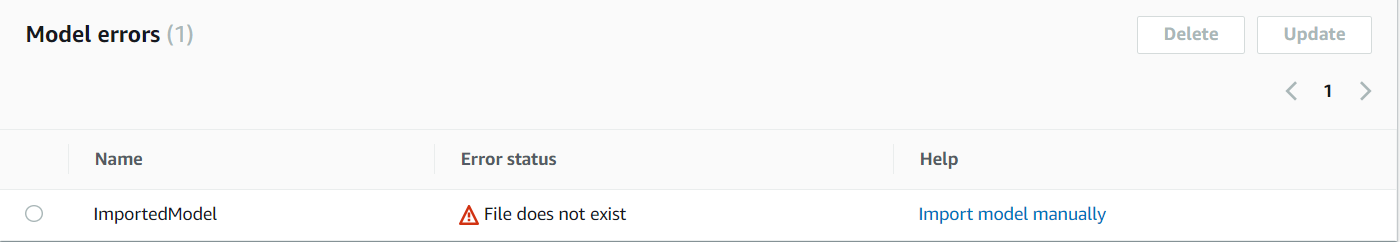
\includegraphics[width=0.9\textwidth]{images/ErrorDuringUpload.PNG}
    \caption[]{Error during import process\footnotemark}
    \label{fig:console-output-start}
\end{figure}
In the above photo, the error message while importing to the garage is shown. The error message is "File does not exist". However, since the orders consist of about 100 files, it is challenging to locate the missing file. This test was done with an S3 bucket, converted to a model in the previous update without any problems. The "Import Model Manually" link leads to a general documentation page that provides rough instructions on how to import Sagemaker models into the s3 bucket, but not how models can be imported into the garage or which file the error message refers to.


\section{Difference between Cloud Training and Local Training}
As expected, the Local training was not performing as good as training in the Cloud. This section will compare the Hardware and Performance of the PC and Cloud. 


\subsection{Performance-Difference}
To precisely measure the difference between the Cloud and the research Computer, a Test-Model was set up. The model specifications are: 
 
\begin{table} [H]
\caption{Sample Model Specifications}
\label{Sample Model Specifications}
\centering
\begin{tabular}{|m{15em}|m{1cm}|}
\hline
\textbf{Hyperparameter} & \textbf{Value} \\
\hline
Gradient descent batch size: & 64 \\
\hline
Entropy: & 0.01 \\
\hline
Discount factor: & 0.999 \\
\hline
Loss type: & Huber \\
\hline
Learning rate: & 0.0003 \\
\hline
Number of experience episodes between each policy-updating iteration: & 20 \\
\hline
Number of epochs: & 10 \\
\hline
\end{tabular}
\end{table}

Using the standard reward function, the model was trained on the Oval Track. This test environment was chosen because it is straightforward to learn, and only given 30 minutes to train the model would not master a more challenging track. Moreover, the Race-Mode was set to time-trial because this model is not trained to race in a league against other Deepracers.
\newline
To compare the two models, and evaluation was started in the AWS-Cloud. This process stimulates the car on the track and drives three laps. Then it determines the probability that the Deepracer will complete a lap without crossing the line.


\subsubsection{Cloud-Training}
After finishing the Evaluation in the Cloud the Results were:

\begin{figure}[H]
    \centering
    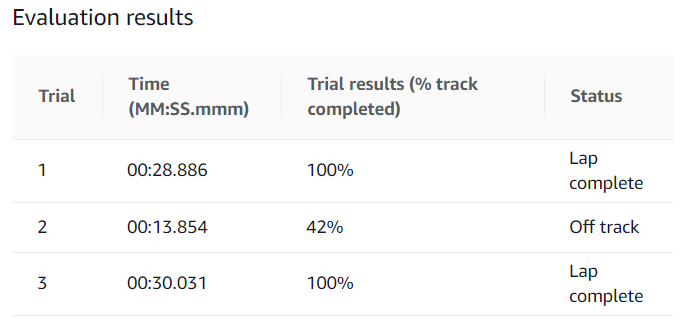
\includegraphics[width=0.9\textwidth]{images/CloudEvaluationResults.PNG}
    \caption[]{Evaluation Results from Cloud Training}
    \label{fig:evRe}
\end{figure}



\subsubsection{Local-Training}
Evaluating the local-Training, the results were as following: 

\begin{figure}[H]
    \centering
    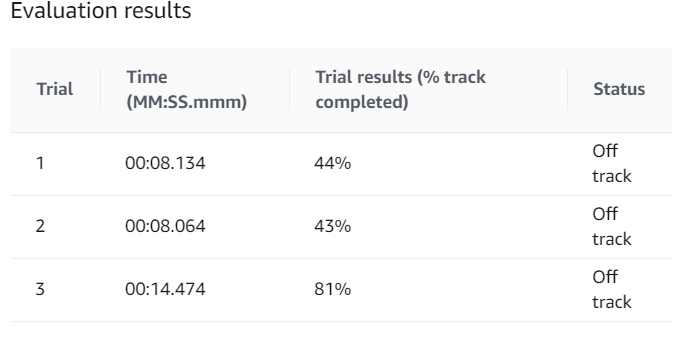
\includegraphics[width=0.9\textwidth]{images/localEvaluation.PNG}
    \caption[]{Evaluation Results from Local Training}
    \label{fig:evLo}
\end{figure}
 
 
\subsection{Price-Difference}
The Table below shows the Difference between storing and evaluating Data online and offline.

\begin{table}[H]
\caption{Pricing for model training with AWS services.}
\label{tab:services}
\centering
\setlength{\tabcolsep}{5mm}
\def\arraystretch{1.25}
\begin{tabular}{|r|r|c|c|}
\hline
\textbf{service} & \textbf{pricing AWS} & \textbf{pricing PC} \\
\hline\hline
training and evaluation & 3.50 US\$ per hour & 0.29 US\$ per hour \\
\hline
model storage & 0.023 US\$ per GB and month & free of charge\\
\hline
\end{tabular}
\end{table}
\footnote{Cited date 2020/08/20}
\repeatfootcite{PowerCost}

\subsection{Price-Example}
To simulate the large price difference, a price example was calculated using students training their Deepracer for 8 hours.

\begin{table}[H]
\caption{Pricing Example}
\label{tab:services}
\centering
\setlength{\tabcolsep}{5mm}
\def\arraystretch{1.25}
\begin{tabular}{|r|r|c|c|}
\hline
\textbf{AWS-DeepRacer-Jobs} & \textbf{Hours} & \textbf{Total PC} & \textbf{Total Cloud} \\
\hline\hline
Training & 8,00 & 2.23 US\$ & 28US\$ \\
\hline
Evaluation & 0.083 & 0 US\$ & 0.29 US\$ \\
\hline
\end{tabular}
\end{table}
\footnote{Cited date 2020/08/20}
\repeatfootcite{PowerCost}

The table above shows, that the total cost for 8 hours of training and evaluation in the Cloud is \$28.29, and on the local PC, it is \$2.23. However, this does not include the purchase of a computer.

\subsection{Result}
After training in the Cloud and training locally, we concluded that the choice depends on the use case. Comparing the training Data, the Cloud is 40\% faster, otherwise comparing the Cost-Explorer, the Cloud is 1268\% more expensive. The AWS-Management Console has very detailed documentation and guides that help the developer to create the first model. It is also effortless and fast to train and evaluate the model. On the other side, local training is very cost-efficient, although it is insufficient and has a poor documentation, the programmer has to have a lot of knowledge of the structure of the Amazon tools and services that are running in the background. 

